\leadauthor{theRmal-landscape}

\title{Variation in thermal pressures and resource availability drives disease dyanmics}
\shorttitle{theRmal-landscape}

\author[1]{
  
% \orcidlink{0000-0001-0000-0000}
}
% \author[2]{Second Doctor \orcidlink {000-0002-0000-0000}}
% \author[1,\Letter]{Third Professor \orcidlink {000-0003-0000-0000}}
% \affil[1]{A University, Academic Street, Learningtown, UK}
% \affil[2]{B Institute, Chalk Road, Blackboardville, USA}
\date{}

% \maketitle

% \begin{abstract}
% Abstract of the paper goes here.
% \lipsum[1]
% \end{abstract}

% \begin{keywords}
% keyword1 | keyword2 | keyword3
% \end{keywords}

% \begin{corrauthor}
% % name\at gmail.com
% \end{corrauthor}

\section*{Brief introduction}\label{s:introduction}

Infectious disease transmission often depends on physical proximity between infected and susceptible individuals, particularly for directly transmitted pathogens. It has been well established in studies of contact networks that the closer these individuals are in space, the greater the likelihood of successful transmission events occurring \citep{proffittElkDistributionSpatial2011}. Understanding what drives this proximity is thus critical for modeling and predicting disease spread. \\

While physical proximity can emerge from complex behavioral and social dynamics, it can also be understood through a simplified ecological lens. In such a framework, individuals make foraging decisions across a heterogeneous landscape, and the probability of disease transmission is tied to the likelihood that multiple individuals co-occupy the same patch at the same time. When an infected and a susceptible host forage in the same location, a direct transmission event becomes possible \citep{whiteUsingContactNetworks2017}. \\

Resource availability is a primary driver of foraging behavior. Individuals are more likely to select habitat patches with higher concentrations of food or other vital resources. However, for many organisms, resource selection is not the only consideration; thermal conditions also play a significant role. In temperature-sensitive species, foraging choices are influenced not just by resource abundance, but by the thermal suitability of patches, which affects metabolic function, activity levels, and survival \citep{tomecekInadequateThermalRefuge2017,nowakowskiChangingThermalLandscapes2018}. \\

Consequently, landscape use and co-location of hosts are driven by a joint interaction between the resource and thermal properties of habitat patches. This means that a simplified but ecologically meaningful model of disease transmission must incorporate both thermal and resource heterogeneity across the landscape. Within this framework, the probability that a single infected individual will transmit a pathogen to another is modulated by the spatial overlap of their foraging decisions, which in turn depends the distribution of acceptable landscape patches for them to choose from. That is, a highly homogeneous landscape in a beneficial way will facilitate lower rates of transmission since organisms can self-assort on the landscape with low probability of occupying the same patch as another infected individual. However, the opposite is also true wherein should the landscape become more heterogeneous those trends will change, and once there are few appropriate locations, co-occurrence probabilities will increase in a way we suspect is highly predictable. \\

In this project, our goal is to formalize this notion about landscape heterogeneity and it's relationship to transmission probabilities. We hope to articulate how transmission dynamics and the probabilities of epidemics spreading are a) dependent on habitat suitability weights, and b) how those suitability weights can be described in terms of both resource availability and thermal tolerability. 


% This framework is particularly relevant for certain biological systems. For example, burrowing organisms that directly transmit pathogens through contact may only interact when selecting the same burrow or feeding ground. In such systems, disease spread is inherently spatial and strongly tied to both the behavioral ecology of the host and the structure of the environment [reference needed].

\section*{Methods \& Results}\label{s:methods-results}

To abstract the transmission dynamics sufficiently, we imagine a landscape where a series of individuals make daily landscape-level selections on where they will forage, with no memory and perfect knowledge of the landscape. Therefore, they chose, independently of other individuals, from the available cells, $w_i$ based on each cell's value as a probability. Since these are probabilities it must be true that 
\begin{equation}
\sum_i w_{i}=1.
\end{equation}

If there are $S$ susceptible individuals in the population that assort randomly across space according to the probabilities $w_{i}$ and $I=1$ infected individual, we want to know the probability that the disease will spread. From a purely contact perspective, this is given by the probability that the infected individual occupies a location that also has at least one susceptible individual.

\subsection{Co-location and transmission}

Assuming a population consisting of $S>0, I>0$, transmission requires at least the co-location of one of each group. We can consider both co-location and transmission.

\subsubsection{Determining the probability that at least one $S$ is located in a cell $i$}

The probability that patch $i$ has zero susceptible individuals is $P(S_{i}=0)=(1-w_{i})^S$, where $S$ is the number of susceptible individuals on the landscape. Thus, the probability that at least one patch at location $i$ has at least one susceptible individual is given by:  
\begin{align}
P(s_{i} \geq 1) &=1-P(s_{i}=0) \\
&=P(s_{i}=1)+P(s_{i}=2)+P(s_{i}=3)+ ... +P(s_{i}=S)
\end{align}
Each of the terms above can be expanded as follows: 
\begin{align}
P(s_{i}=k)=\binom{S}{k}w_{i}^k(1-w_{i})^{S-k}
\end{align}
and therefore
\begin{align}
P(s_{i} \geq 1)&=\sum_{k=1}^{S}\binom{S}{k}w_{i}^k(1-w_{i})^{S-k}\\
&=\left((1-w_{i})^{-S}-1\right)(1-w_{i})^S\\
&=1-(1-w_{i})^S
\end{align}

\subsubsection{Joint Probability for Co-location of $S$ and $I$}
For disease spread to occur, both a susceptible individual and an infected individual must be in the same cell. The probability of this is the product of the independent events:
\begin{equation}
P(\text{collocation in cell } i) = P(S_{i} \geq 1) \cdot P(I_{i} \geq 1).
\end{equation}

Expanding this:
\begin{equation}
P(\text{collocation in cell } i) = \left[ 1 - (1 - w_{i})^S \right] \cdot \left[ 1 - (1 - w_{i})^I \right].
\end{equation}
which, if we assume instead of $I\geq1$ that $I=1$ then this becomes
\begin{equation}
P(\text{collocation in cell } i) = \left[ 1 - (1 - w_{i})^S \right] \cdot w_i.
\end{equation}

\subsection{Landscape with a known distribution}

\subsubsection{Assuming constant values}

In order to verify that our expectation accurately captures the simulated version of the landscape, we can compare the two. First, we assume that we know the values/distribution of the landscape itself. The landscape on which individuals are making occupancy decisions can be thought of as consisting of normalized values. We also focus on the case where there is only one $I$ individual and transmission is assured by co-occurring on the landscape.

First, we assume that the weights on the landscape are all equal, and there are $n=100$ patches, and $I=1$ infected individuals. In this case, the expected number of co-occurrences ($CO$) is given as 

\begin{equation}
    E[CO] = (S+I)(1-(1-\frac{1}{n})^S
\end{equation}

We simulate this process using a simple random choice based on constant values of $w$, and show that the expected values track the simulated values very well \cref{fig:constant}, which is to be expected.

\begin{figure}[!hpt]
    \centering
    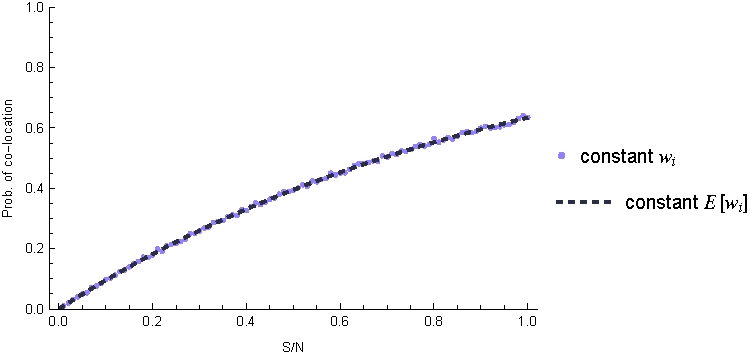
\includegraphics[width=0.75\linewidth]{figs/si/constant-expected.pdf}
    \caption{Expected and simulated values from constant uniform distribution.}
    \label{fig:constant}
\end{figure}

\subsubsection{Assuming values come from a known distribution}

Ideally we can describe a closed form solution that gives the expected values when the values of $w$ are not constant but are drawn from a known, described distribution.

We begin considering that $w$ takes a uniform random distribution. We assume that the quality $q_i$ of each patch is drawn at random from a uniform distribution $(0,1)$, and then transform these qualities to get patch weights $w_i$ by dividing each patch by the total of the quality values where $i = 1,...,n$. 

\begin{equation}
    w_i = \frac{q_i}{\sum_i{q_i}}
\end{equation}

Here, $w_i$ are therefore nearly uniformly distributed 
\begin{equation}
    (0, \frac{2}{n})
\end{equation} 
for large enough $n$. Here we are considering the case where co-location by two $S$ individuals is given by 
\begin{equation}
    n*w(1-(1-w)^S).
\end{equation} 

If we assume that $n>2$ and also that $S \geq 1$, then the expectation of our co-location is: 

\begin{equation}
    E[n*w(1-(1-w)^S)] = \frac{n^{-S} \left(\left(2 (S+1) (S+2)-n^2\right) n^S+(n-2)^{S+1} (n+2
   S+2)\right)}{2 (S+1) (S+2)}. 
   \label{eq:uniform-expectation}
\end{equation}

If we compare this set of expected values, varying the ratio of $S/n$, then we can see our expected values match the draws from a simulated distribution \cref{fig:constant-uniform}.

\begin{figure}[!hpt]
    \centering
    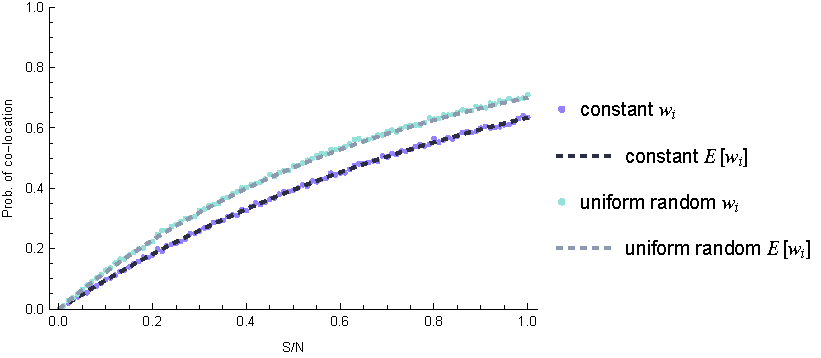
\includegraphics[width=0.8\linewidth]{figs/si/constant-uniform.pdf}
    \caption{Expected and simulated values from constant uniform and uniform random expectations.}
    \label{fig:constant-uniform}
\end{figure}

We could also assume that the weights are exponentially distributed, since $n$ random draws from an exponential with a mean $\frac{1}{\lambda} = 1$ would sum to a mean of 1, given large enough $n$. That would take the form 

\begin{equation}
    E[n*w(1-(1-w)^S)] = \frac{1-n^2+S-\mathcal{e}^{-n}(-n)^{-S}(1+n+S)((-1+(-1)^{2S}) \Gamma(2+S)+\Gamma(2+S, -n))}{1+S}
    \label{eq:exp-expectation}
\end{equation}

which does have a closed form, though it is unwieldy. However, this result follows the uniform random assumption and shows a close following of the simulated results to the expected results \cref{fig:const-uni-exp}

\begin{figure}[!hpt]
    \centering
    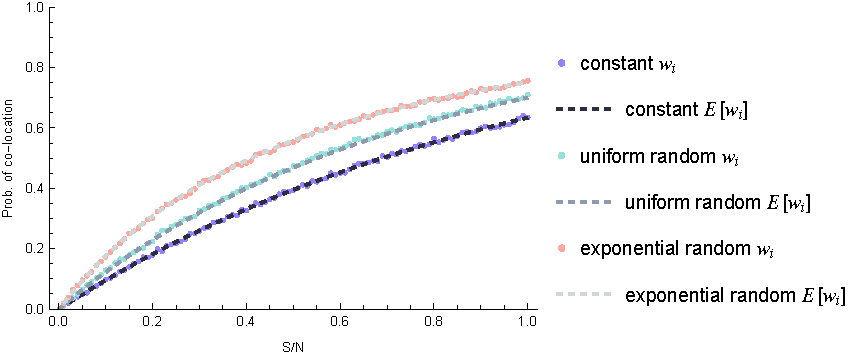
\includegraphics[width=0.8\linewidth]{figs/si/constant-uni-exp.pdf}
    \caption{Expected and simulated values from constant uniform, uniform random, and exponential random expectations.}
    \label{fig:const-uni-exp}
\end{figure}

Other distributional assumptions could possibly made, but the decidedly in-elegant forms of the uniform and exponential distributions make the likelihood of additional distributions showing easy to interpret expressions.

\subsection{Probability of Successful Transmission on a Realistic Landscape}

To determine whether or not transmission can occur, we consider the case where infected and susceptible individuals are present on the same landscape patch, and also the likelihood of a transmission event occurring successfully. We denote this as $\epsilon(T)$ which is the temperature dependent probability of transmission.  Given some collocation, if there is some patch with $S = 1, I = 1$, the likelihood of transmission is just $\varepsilon_{i}(T)$. In the case of $S = 2$, we have the probability of 
\begin{align}
    \text{At least one S getting infected} &\rightarrow 1 - (1- \varepsilon(T))^2, \\
    \text{Both } S \text{ getting infected} &\rightarrow \varepsilon(T)^2, \text{and} \\
    \text{Neither } S \text{ getting infected} &\rightarrow (1 - \varepsilon(T))^2
\end{align}

\subsubsection{Some number of susceptible individual and one infected} \\

If there is only $I = 1$ then the probability of at least one of the susceptible $k$ undergoing infection, $P^*(S, I)$ is

\begin{equation}
    P^*(k, I=1) = \sum^{k=S}_{k = 1}\begin{pmatrix} S\\ k \end{pmatrix} w(T)^{k-1}(1-w(T))^{S-k}(1 - (1-\varepsilon(T))^k)
\end{equation}

From there we can understand that the probability of a disease spreading on the landscape from cell $i$, $\phi_{i}(k, I = 1)$ is 

\begin{equation}
    \phi_{i}(k, I = 1) = 1 - (1 - w(T) \varepsilon(T))^S
\end{equation}

And therefore, the probability of it spreading on the landscape at all is:

\begin{equation}
    \boldsymbol{\phi}(k, I = 1) = \sum_i 1 - (1 - w(T) \varepsilon(T))^S
\end{equation}

\subsubsection{Landscape choice based on temperature and resource levels}

If we consider a landscape where now the values of $w_{i}$ are given by not a known distribution, but the functional response of organisms to the temperature and resource supply on the landscape, then we can create a more realistic environment. We can say that the landscape values are given by

\begin{equation}
    w_{i} = \text{Max}(0, f(T_{i}, R_{i}))
\end{equation}

where $f(T_{i}, R_{i})$ is the function defining the suitability of patch $i$ based on the resource availability and temperature suitability of patch $i$:

\begin{equation}
    f(T_{i}, R_{i}) = \frac{I_{\text{max}}(T_{i} R_{i})}{R_{i} + R_{\text{half}}} - m(T_{i}),
\end{equation}

with $m(T)$ being a respiration term of the organism, and $I_{\text{max}(T)}$ is the maximum uptake rate, where $m(T) = m_a e^{m_b \times T} + m_c$ and $I_{\text{max}}(T) = e^{-(T - T_I)^2 / \gamma}$ with $m$ being an approximated exponential version of the Boltzmann-Arrhenius relationship. Here $T_I$ is the optimal temperature value and $\gamma$ determines the breadth of the response. This value is dependent on each cell, where $T_{i}$ is the temperature value at $i$ and $R_{i}$ is the inflow supply of some resource for the organism choosing it's location \cref{fig:t-s-wij-grid}. The values for a given cell of $T$ and $S$ are drawn from:

\begin{align} \label{eq:s-t}
    T_{i} \sim \mathcal{N}(\mu_T, \sigma_T) \\
    R_{i} \sim \mathcal{N}(\mu_R, \sigma_R)
\end{align}

which produce the distributions shown in \Cref{fig:t-s-wij-grid}:

\begin{figure}[!hpt]
    \centering
    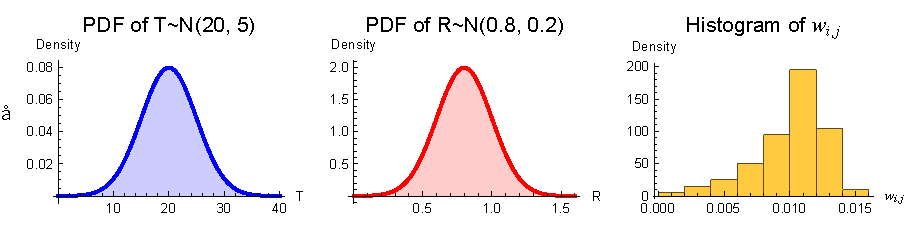
\includegraphics[width=0.99\linewidth]{figs/si/R-T-pdfs-W-hist.pdf}
    \caption{Distributions for $T$, $R$, and $w_i$}
    \label{fig:t-s-wij-grid}
\end{figure}

We can then simulate $\Phi$ for a landscape, which results in a set of results like \Cref{fig:landscape-trans}.

\begin{figure}[!hpt]
    \centering
    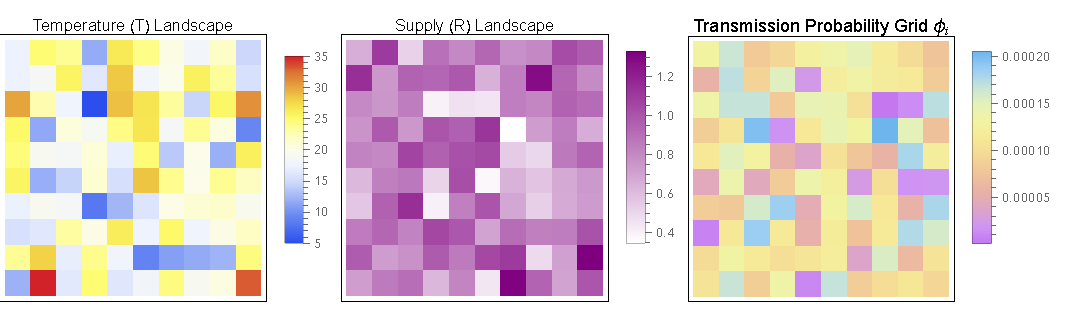
\includegraphics[width=0.8\linewidth]{figs/si/temp-supply-probability-landscape.pdf}
    \caption{Landscape-level probability of transmission occurring.}
    \label{fig:landscape-trans}
\end{figure}

and an overall $\phi(k=1, I=1)$, where with $n = 100$, $\mu_T = 20$, $\mu_R = 0.8$, $\sigma_R = 0.2$, $\sigma_T = 5$, and $\epsilon=1$, the $\phi = 0.0107249$

\section*{Where we want to go}

As it currently stands, we can start to try and understand on a realistic landscape how factors such as temperature and supply may affect co-occurence probabilities, but from a more theoretical standpoint, we are limited in what we can say. Currently, we have come up with expressions (e.g. \cref{eq:exp-expectation,eq:uniform-expectation}) that allow us to determine whether or not, given some known number of locations $n$ and the number of susceptible individuals $S$, how likely a co-occurrence (and therefore transmission event) is to happen. However, so far: 
\begin{itemize}
    \item We cannot say anything concrete about what happens when $I=2$.   We know that the probability of co-occurrence will increase compared to the case of $I=1$ (for reasonably large $S$), but there is still some chance that it will fail at each step.  
    \item This will also depend on the period of infectiousness (e.g how many re-assortments of the landscape occur before death or recovery of $I$).
    \item The expressions we have are decently complex and don't offer much by way of elegant explanation 
\end{itemize}

Ultimately, we'd like to find a way to come up with an closed-form probability statement that allows us to say something along the lines of ``We are 95\% certain that an epidemic will spread under these conditions.'' This would mean that we could say, given a particular landscape weight $w$ distribution, number of $S$, number of total organisms $N$ and number of locations $n$, we could come up with an expectation that, for example, at least 50\% or even 100\% of the organisms will become infected. This would of course be assuming no loss of infection nor death (i.e. there is no recovery term either to a recovered state ($R$), nor back to the $S$ state. Additionally, $N$ is assumed to stay the same through the course of the process.

\section*{Calculating $R_0$ from our model}

It turns out we can derive the connection between our model (where we've been) with the expected $R_0$ quite easily.  If we begin by assuming that there are $I=1$ infected individuals in the population and $S$ susceptible individuals then the expected number of new infections arising in the first step $I_{new}$ (assuming that the infected individual lives for only one time step) is weighted averages of the co-occupancy probabilities: 

\begin{align}
R_0=E[I_{new}]&=\sum_{i=1}^{n}[ 0\cdot P(I=1 \text{ in }i) \cdot P(S=0 \text{ in }i) \\
&+1\cdot P(I=1 \text{ in } i) \cdot P(S=1 \text{ in }i) \\
&+2\cdot P(I=1 \text{ in } i) \cdot P(S=2 \text{ in }i) \\
&+ \dots\\
&+S\cdot P(I=1 \text{ in } i) \cdot P(S=S \text{ in }i)] \\
&\\
&=\sum_{i=1}^{n}\sum_{k=0}^S k \cdot w_i \cdot \binom{S}{k}w_i^k(1-w_i)^{S-k}
\end{align}

Here the variable $k$ sums across the $S+1$ different possible numbers of susceptible individuals in a patch.   We assume that co-occupancy leads to infection however adding an additional parameter could be added to reflect differences in infection probabilities among patches.   

If we assume constant patch occupancy probabilities such that $w_i=w=1/n$ then
\begin{align}
R_0=E[I_{new}]&=n \cdot S \cdot w^2\\
&=S/n
\end{align}

If we assume that patch occupancy probabilities are uniformly distributed on the interval $(0,2/n)$, for large enough $n$ their sum converges to 1 (satisfying their use as weights) and 
\begin{align}
R_0=\frac{4S}{3n}
\end{align}

We can even take this one step further to show that any variation among patches will increase $R_0$. If we assume that occupancy probabilities are uniformly distributed on the interval $w \approx  \mathcal{U}(1/n-q,1/n+q)$ then $q\rightarrow0$ corresponds to the case of a constant patch weight and increasing $q$ on the interval $0<q\leq 1/n$ represents an increase in the variance of the landscape.  The solution of $R_0$ is

\begin{align}
R_0=\frac{S}{n}+n S \frac{q^2}{3}
\end{align}

where $q^2/3$ is the variance of $\mathcal{U}$.  When $q=1/n$ (which is the limiting case because patch weights cannot be less than zero), we can see why the fraction $4/3$ emerges in the solution on line 36. 

If we assume that patch occupancy probabilities are exponentially distributed with mean $1/n$,

\begin{align}
R_0=\frac{2S}{n}
\end{align}

We cannot do the same variance expansion with the exponential distribution that we did with the uniform.   

%\section*{Results}\label{s:results}


%\section*{Discussion}\label{s:discussion}

\section*{Bibliography}
\bibliographystyle{bxv_abbrvnat}
\bibliography{theRmal-landscape}
